\newpage

\subsection{A Cram\'{e}r-Lundberg process with a matrix exponential density} \label{e:MatExp6220}

Next we consider an example produced by taking a Cram\'{e}r-Lundberg process with matrix exponential density of claims $f(x)=\a e^{A x} (-A) \bff 1 $, where $\a=(-2.4, 0.9 , 2.5),  A = \bep
   {-6.2, 2, 0}\\
   {2, -9, 1}\\
   {1, 0, -3}\eep$
and $\l=1$, $\th=1$, $q=\fr{1}{10}$.

The Laplace exponent of this process is
$\kappa(s) = 1.3249 s -\frac{3.34053 s}{s+2.87761}+\frac{3.03143 s}{s+5.34047}-\frac{0.690902 s}{s+9.98192}$ and the scale function is
\bea
W_q(x)  &= -0.0655864 e^{-9.35143 x}+0.149742 e^{-6.89805 x}-0.676982 e^{-1.26245 x}+1.3476 e^{0.142175 x}.
\eea

\begin{figure}[!h]
    \centering
    \begin{subfigure}[b]{0.8\textwidth}
        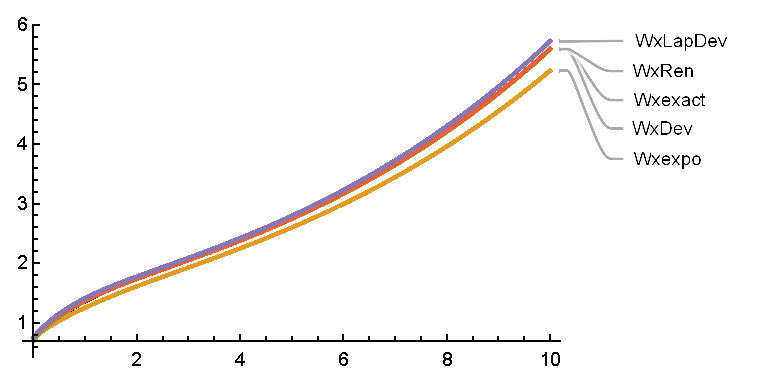
\includegraphics[width=\textwidth]{MatExp6220W}
        \caption{$W_q(x)$  (in black)}
        \label{fig:MatExp6220W}
    \end{subfigure}
    ~
    \\
    \begin{subfigure}[b]{0.8\textwidth}
        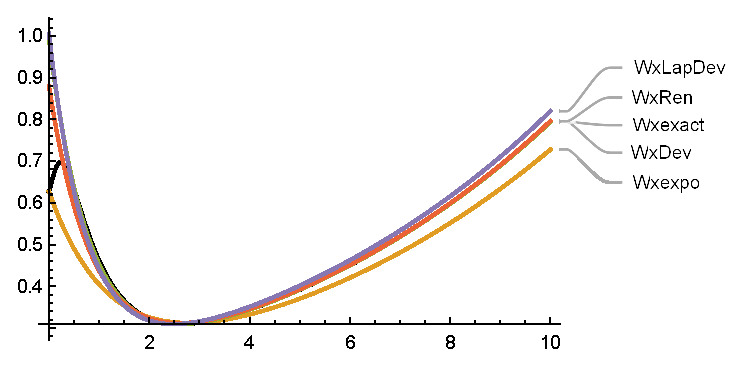
\includegraphics[width=\textwidth]{MatExp6220W1}
        \caption{$W'_q(x)$}
        \label{fig:MatExp6220W1}
    \end{subfigure}
    ~
    \\
    \begin{subfigure}[b]{0.8\textwidth}
        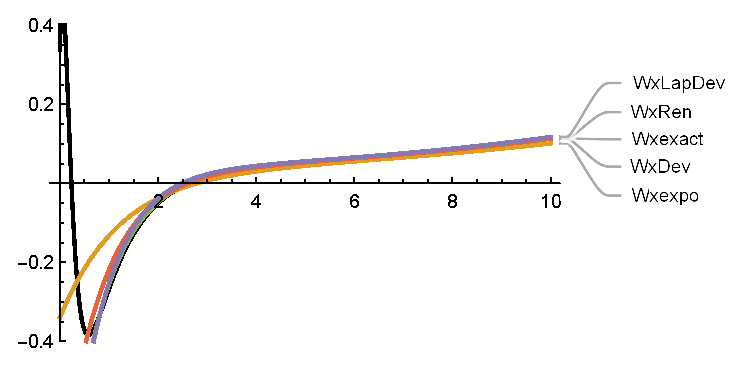
\includegraphics[width=\textwidth]{MatExp6220W2}
        \caption{$W''_q(x)$}
        \label{fig:MatExp6220W2}
    \end{subfigure}
    \caption{Plots of $W_q(x)$, $W'_q(x)$, and $W''_q(x)$ of the exact solution and the approximations for $f(x)=\a e^{A x} (-A) \bff 1 $, $\th=1$, $q=\fr{1}{10}$.}\label{fig:MatExp6220}
\end{figure}


\begin{table}[!h]
\begin{tabular}{|l|l|l|l|l|}
\hline
       & \begin{tabular}[c]{@{}l@{}}Dominant   exponent \\ $\Phi_q$\end{tabular} & \begin{tabular}[c]{@{}l@{}}Percent   relative error\\ ($\Phi_q$)\end{tabular} & \begin{tabular}[c]{@{}l@{}}Optimal barrier\\ $b_{DeF}$\end{tabular} & \begin{tabular}[c]{@{}l@{}}Percent   relative error\\ ($b_{DeF}$)\end{tabular} \\ \hline
Exact  & 0.142175                   & 0                                 & 2.61925              & 0                             \\ \hline
Expo   & 0.139202                   & 2.09118                           & 2.79162              & 6.58074                       \\ \hline
Dev    & 0.142174                   & 0.00104491                        & 2.60329              & 0.609153                      \\ \hline
Renyi  & 0.142238                   & 0.0439717                         & 2.59638              & 0.873044                      \\ \hline
LapDev & 0.143232                   & 0.743272                          & 2.48327              & 5.19155                       \\ \hline
\end{tabular}
\caption{Exact and approximate values of $\Phi_q$ and $b_{DeF}$ for $f(x)=\a e^{A x} (-A) \bff 1 $, $\th=1$, $q=\fr{1}{10}$. The DeVylder approximation displayed the least percent relative error among the four approximations considered.}
\label{table:MatExp6220}
\end{table}


\begin{table}[!h]
\begin{tabular}{|l|l|l|l|l|}
\hline
$\theta$ & Closest approximation & $\Phi_q$   exact & $\Phi_q$ approximation & \% error   $\Phi_q$ \\ \hline
1   & Dev                     & 0.142175       & 0.142174 & 0.00104491        \\ \hline
0.9 & Dev                     & 0.156039       & 0.156036 & 0.00148235        \\ \hline
0.8 & Dev                     & 0.172688       & 0.172684 & 0.00216274        \\ \hline
0.7 & Dev                     & 0.192979       & 0.192973 & 0.00325715        \\ \hline
0.6 & Dev                     & 0.218117       & 0.218106 & 0.0050835         \\ \hline
0.5 & Dev                     & 0.249825       & 0.249804 & 0.0082542         \\ \hline
0.4 & Dev                     & 0.290594       & 0.290553 & 0.013988          \\ \hline
0.3 & Dev                     & 0.344047       & 0.343962 & 0.0247701         \\ \hline
0.2 & Dev                     & 0.415404       & 0.415214 & 0.0457098         \\ \hline
0.1 & Dev                     & 0.512          & 0.511554 & 0.0871333         \\ \hline
\end{tabular}
\caption{Exact and approximate values of $\Phi_q$ for $f(x)=\a e^{A x} (-A) \bff 1 $, varying the value of $\theta$. The DeVylder approximation displayed the least percent relative error among the four approximations considered.}
\label{table:MatExp6220Phiq}
\end{table}



\begin{table}[!h]
\begin{tabular}{|l|l|l|l|l|}
\hline
$\theta$ & Closest approximation & Barrier exact & Barrier approx & \% error Barrier \\ \hline
1   & Dev                     & 2.61925         & 2.60329  & 0.609154           \\ \hline
0.9 & Dev                     & 2.52243         & 2.50437  & 0.716072           \\ \hline
0.8 & Expo                    & 2.39997         & 2.39528  & 0.195427           \\ \hline
0.7 & Dev                     & 2.24344         & 2.22233  & 0.941111           \\ \hline
0.6 & Dev                     & 2.04159         & 2.01986  & 1.06465            \\ \hline
0.5 & Dev                     & 1.77996         & 1.75855  & 1.20296            \\ \hline
0.4 & Dev                     & 0               & 1.4216   & -                  \\ \hline
0.3 & Expo                    & 0               & 0.518511 & -                  \\ \hline
0.2 & Exact                   & 0               & 0        & -                  \\ \hline
0.1 & Exact                   & 0               & 0        & -                  \\ \hline
\end{tabular}
\caption{Exact and approximate values of $b_{DeF}$ for $f(x)=\a e^{A x} (-A) \bff 1 $, varying the value of $\theta$.  The DeVylder approximation displayed the least percent relative error among the four approximations considered.}
\label{table:MatExp6220Bar}
\end{table}